\documentclass[main]{subfiles}

\begin{document}

\chapter{Hardware}
La elecci\'on del hardware representa una parte muy importante del Proyecto. Una mala elecci\'on de alguno de los componentes puede acarrear complicaciones no previstas a la hora de la ejecuci\'on, causando contratiempos inesperados y trabajo excesivo. Es necesario, entonces, el estudio detallado de cada uno de los componentes a utilizar.

\section{Plataforma f\'isica: Cuadric\'opteros}

\begin{wrapfigure}{r}{0.4\textwidth}
\vspace{20pt}
	\centering
	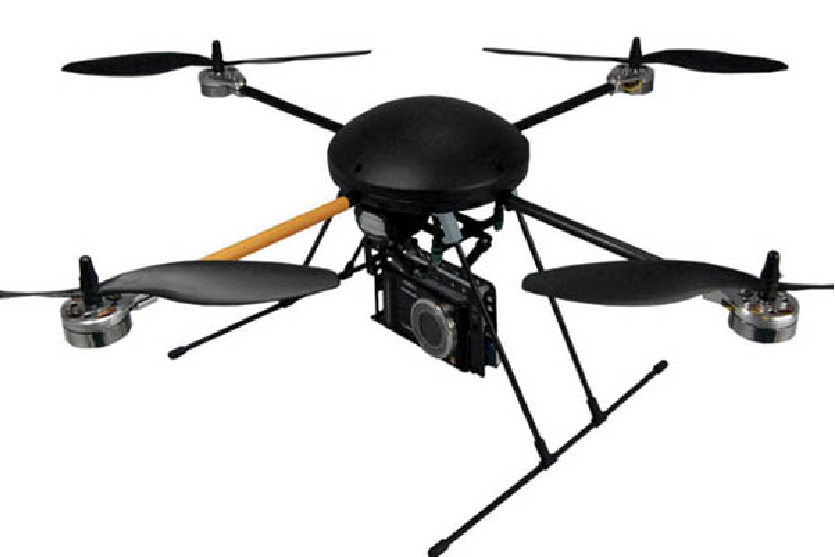
\includegraphics[width=0.35\textwidth]{./pics_eleccion_hardware/turboace.png}
	\caption{Turbo Ace X720}
	\label{fig:cuadricoptero}
\vspace{20pt}
\end{wrapfigure}

A la hora de la planificaci\'on del Proyecto se plantea la opci\'on de partir de cero, dise\~nando completamente el cuadric\'optero. Si bien esta opci\'on tiene la ventaja de que se puede conocer completamente su funcionamiento, implica problemas de ingenier\'ia mec\'anica que no se pretenden resolver, conocimientos de resistencia, flexibilidad y peso de materiales, as\'i como tambi\'en diversas complicaciones adicionales a la hora de fabricar y armar los distintos componentes. Dados los plazos del proyecto, y que su objetivo se centra en el control del veh\'iculo, la necesidad de partir de un dispositivo electromec\'anico ya construido resulta imperiosa.\\

La plataforma escogida es el cuadric\'optero \textbf{Turbo Ace X720}. Esta plataforma es controlada por un usuario a trav\'es de un control remoto comercial est\'andar (Walkera 2801). El sistema receptor se encarga de \emph{setear} la velocidad angular de cada motor en funci\'on de la se\~nal recibida.\\

La plataforma escogida consta de un receptor, una CPU, una batería, 4 motores y 4 ESCs\footnote{Electronic Speed Controller} montados sobre un cuerpo de fibra de carbono. Además incluye un transmisor (control remoto), imprescindible para volarlo. La electrónica original (ESCs y CPU) también se puede encontrar bajo el nombre de \textbf{Lotus RC T580}, otra plataforma comercial.

\subsection*{Motores}
Los motores de la plataforma son de tipo \emph{Brushless} (sin escobillas): son el\'ectricos con el rotor de im\'an permanente y tres pares de bobinas en el estator alimentados con corriente continua conmutada. Necesitan de un sistema de conmutaci\'on el\'ectrico (\textbf{ESC}) que los controlen, y presentan relaciones lineales entre corriente y torque, y entre frecuencia y velocidad. Son com\'unmente utilizados en veh\'iculos radio-controlados por su eficiencia, potencia, durabilidad y su bajo peso (en comparaci\'on con los de tipo \emph{Brushed}).\\

Como se explica en \cite{bib:brushless}, la energía eléctrica es convertida a mecánica mediante las fuerzas de atracción magnéticas entre el imán permanente del rotor y el campo magnético giratorio inducido por los devanados del rotor. En la figura \ref{fig:brushless}, también tomada de \cite{bib:brushless}, se muestra un diagrama simplificado de un motor \emph{Brushless}.

\begin{figure}[h!]
%\vspace{-10pt}
	\centering
	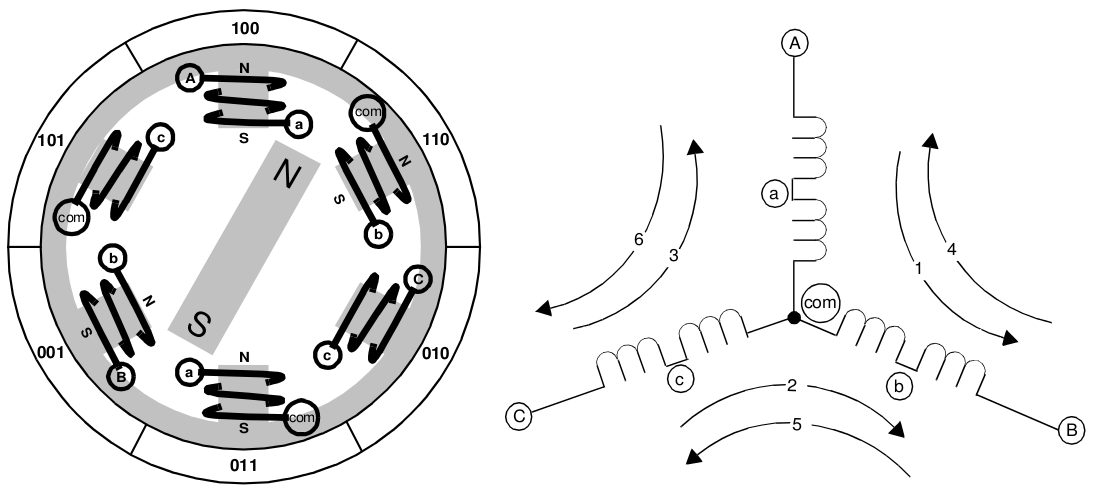
\includegraphics[width=0.7\textwidth]{./pics_eleccion_hardware/brushless.png}
\vspace{-10pt}
	\caption{Esquema simplificado de motor \emph{Brushless}}
	\label{fig:brushless}
\end{figure}

En este ejemplo se muestran 3 circuitos electromecánicos conectados a un punto común y separados en el centro para permitir el movimiento del rotor. La mayoría de los motores \emph{Brushless} tienen un devanado en 3 fases con topología de estrella, como se muestra en la figura anterior. Un motor con esta topología se maneja energizando 2 de las fases al mismo tiempo. Para energizar en el momento adecuado cada pareja de fases se utiliza un controlador electrónico de velocidad, como se explicó anteriormente.

\subsubsection*{Controlador electrónico de velocidad (ESC)}

Los ESCs inclu\'idos en la plataforma reciben comandos mediante el protocolo $I^2C$, a $333kHz$. Se encargan de conmutar la corriente continua que reciben los motores de modo de energizar la pareja de fases correspondiente en el momento justo para que el campo electromagnético inducido genere el máximo torque posible sobre el imán del rotor. En la práctica el máximo torque es alcanzado cuando el imán permanente del rotor está desfasado $90^o$ respecto del campo magnético resultante en el rotor.

La clave del funcionamiento de un motor \emph{Brushless} es poder sensar la posición del rotor y en función de ello energizar las fases que ejercerán mayor torque. Para dicho sensado comúnmente se utiliza un sensor de posición de 3 elementos basado en el \emph{efecto Hall}.\\

El rotor se mueve 60 grados por cada paso de la conmutación. La ruta apropiada para la corriente del estator es activada cuando el rotor se encuentra a $120^o$ de la dirección del campo magnético del estator y es desactivada cuando el rotor pasa $60^o$ dicha dirección, momento en el cual se activa el siguiente circuito y se repite el proceso. En cada instante una de las fases del motor es conducida a nivel alto, otra a nivel bajo y la restante se deja ``flotando''.\\

\begin{wrapfigure}{l}{0.44\textwidth}
\vspace{-20pt}
	\centering
		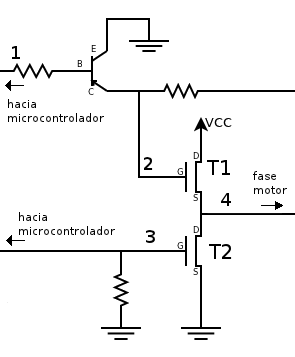
\includegraphics[width=0.38\textwidth]{./pics_eleccion_hardware/bldc_control.png}
\vspace{-10pt}
	\caption{Conmutación BLDC}
	\label{fig:bldc_control}
\end{wrapfigure}

Para realizar la conmutación se utiliza una configuración conocida como ``puente H'', donde por cada fase se utilizan 2 transistores encargados de conducir a los niveles alto y bajo y un tercer transistor (\emph{driver}) que maneja al primero. En la figura \ref{fig:bldc_control} se muestra un diagrama típico de un circuito utilizado para conmutar corriente continua en una fase de un motor \emph{Brushless}. Una precaución muy importante que se debe considerar para este tipo de motores es no activar nunca al mismo tiempo los caminos al nivel bajo y al nivel alto, es decir que nunca conduzcan al mismo tiempo los transistores \emph{T1} y \emph{T2}. Los estados viables para los transistores son las mostradas en la tabla \ref{tab:estado_transistores}.\\

\begin{table}[H]
\begin{center}
\rowcolors{1}{gray!20}{}
\vspace{-10pt}
\begin{tabular}{|c|c|c|c|}
\hline
\textbf{Configuración} & \textbf{T1} & \textbf{T2} & \textbf{Fase} \\ \hline
A & Cortado & Cortado & Flotando \\
B & Conduciendo & Cortado & Nivel alto \\
C & Cortado & Conduciendo & Nivel bajo \\
\hline
\end{tabular}
\caption{Configuraciones posibles para los transistores}
\vspace{-20pt}
\label{tab:estado_transistores}
\end{center}
\end{table}

Si se impone un voltaje mayor a $0.7 V$ en la base del \emph{driver} (punto \textbf{1} de la figura \ref{fig:bldc_control}), dicho transistor conducirá, lo cual fijará un voltaje de $0.2V$ en el punto \textbf{2} del diagrama, correspondiente al \emph{gate} del transistor \textbf{T1}. Este voltaje en el \emph{gate} provoca que el transistor quede cortado, no dejando pasar corriente entre el \emph{source} y el \emph{drain}. En esta situación hay 2 escenarios posibles: que el transistor \textbf{T2} se encuentre conduciendo o que se encuentre cortado. Para que se de el primer escenario (configuración \textbf{C}) es necesario que el microcontrolador imponga un voltaje positivo en el gate del transistor \textbf{T2}, logrando un camino de baja impedancia entre tierra y la fase en cuestión del motor. En este caso se estaría conduciendo dicha fase a nivel bajo. El otro escenario implica que dicha fase quede en estado ``flotando'' (configuración \textbf{A}) ya que ambos transistores permanecen cortados. Por último la otra situación posible es que el transistor \textbf{T1} conduzca (configuración \textbf{B}), situación en la cual el transistor \textbf{T2} deberá permanecer cortado, lo cual se logra llevando a $0V$ el punto \textbf{1} del diagrama.\\

\begin{figure}[h!]
	\centering
	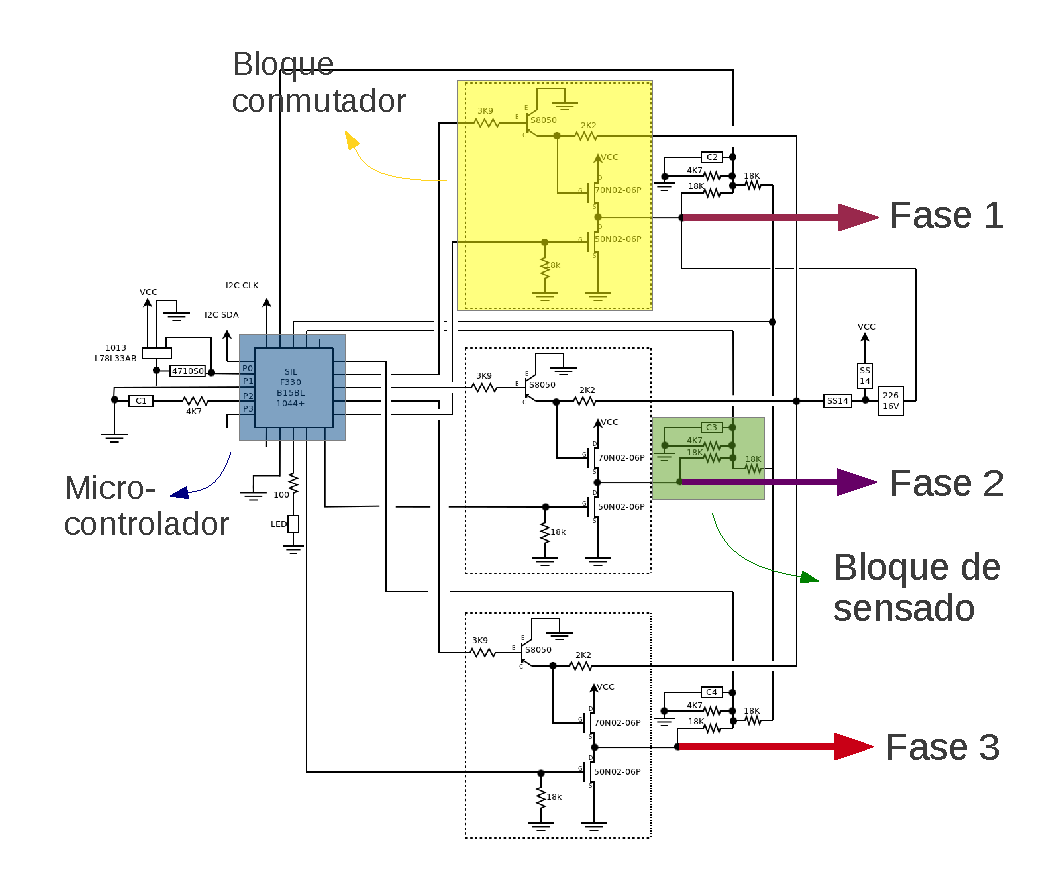
\includegraphics[width=1\textwidth]{./pics_eleccion_hardware/diagrama_ESC.pdf}
	\vspace{-10pt}
	\caption{Esquemático de un ESC}
	\label{fig:diagrama_esc}
\end{figure}

En la figura \ref{fig:diagrama_esc} se muestra el diagrama de un ESC obtenido al relevar el controlador que originalmente incluía el cuadricóptero comercial adquirido\footnote{Este controlador se dej\'o de fabricar, existen dos versiones nuevas de ESC, una de ellas mantiene el mismo protocolo de comunicaci\'on que el aqu\'i presentado, esto fue verificado, ya que en la \'ultima versi\'on de la plataforma implementada se utiliz\'o este controlador.  Los fabricantes indican que hay la otra versi\'on utiliza un protocolo de comunicaci\'on distinto, no se trabaj\'o con estos ESC. }. Se pueden identificar los diversos bloques mencionados a los largo de esta sección. El bloque se sensado es utilizado para obtener la posición del rotor en cada instante de tiempo, el bloque de conmutación es el encargado de energizar las fases correspondientes en cada paso y microcontrolador es el encargado de interpretar la información del sensado de la posición del rotor y actuar sobre los transistores para generar el campo magnético rotatorio. Las fases \textbf{1}, \textbf{2} y \textbf{3} se conectan a los terminales \textbf{A}, \textbf{B} y \textbf{C} mostrados en la figura \ref{fig:brushless}. El denominado ``puente H'' se forma entre cada pareja de bloques de conmutación y las bobinas del motor que quedan energizadas.

\subsubsection*{Instrumentaci\'on e inteligencia}

	La instrumentaci\'on con la que cuenta el dispositivo est\'a destinada a simplificar el manejo a control remoto, estabilizando el sistema. La misma incluye un bar\'ometro y aceler\'ometro y gir\'oscopo de 3 ejes. Cuenta adem\'as con una CPU que se encarga de la lectura de los datos proporcionados por los sensores y de definir las acciones de control sobre los motores. No se dispone del c\'odigo del programa presente en la CPU, y por lo tanto no es posible reutilizarlo, ni tampoco obtener la lectura de los sensores presentes. Se realizaron esfuerzos para conseguir dicha informaci\'on del fabricante, quien se neg\'o a proporcionarla. Por dicho motivo se opta por dotar al sistema de instrumentaci\'on adicional. 

\subsubsection*{Tiempo de vuelo}

El tiempo de vuelo utilizando una bater\'ia de LiPo de 5300mAh (450g) y una carga de 500g es cercano a los 10-15 minutos.

\subsubsection*{Carga \'util}

Adem\'as de toda la instrumentaci\'on que incluye el cuadric\'optero, se incorporar\'a una placa de desarrollo, una de sensores (IMU), un GPS, una interfaz para comunicaci\'on Wi-Fi, y una bater\'ia dedicada exclusivamente a alimentar la electr\'onica agregada. Es de inter\'es conservar la posibilidad de integrar una c\'amara fotogr\'afica. La carga que puede levantar el cuadric\'optero es de 1300g, de la que se debe descontar el peso de las bater\'ias de la electr\'onica y de la alimentaci\'on a los motores.


\section{Inteligencia}
\begin{wrapfigure}{l}{0.35\textwidth}
\vspace{-30pt}
	\centering
	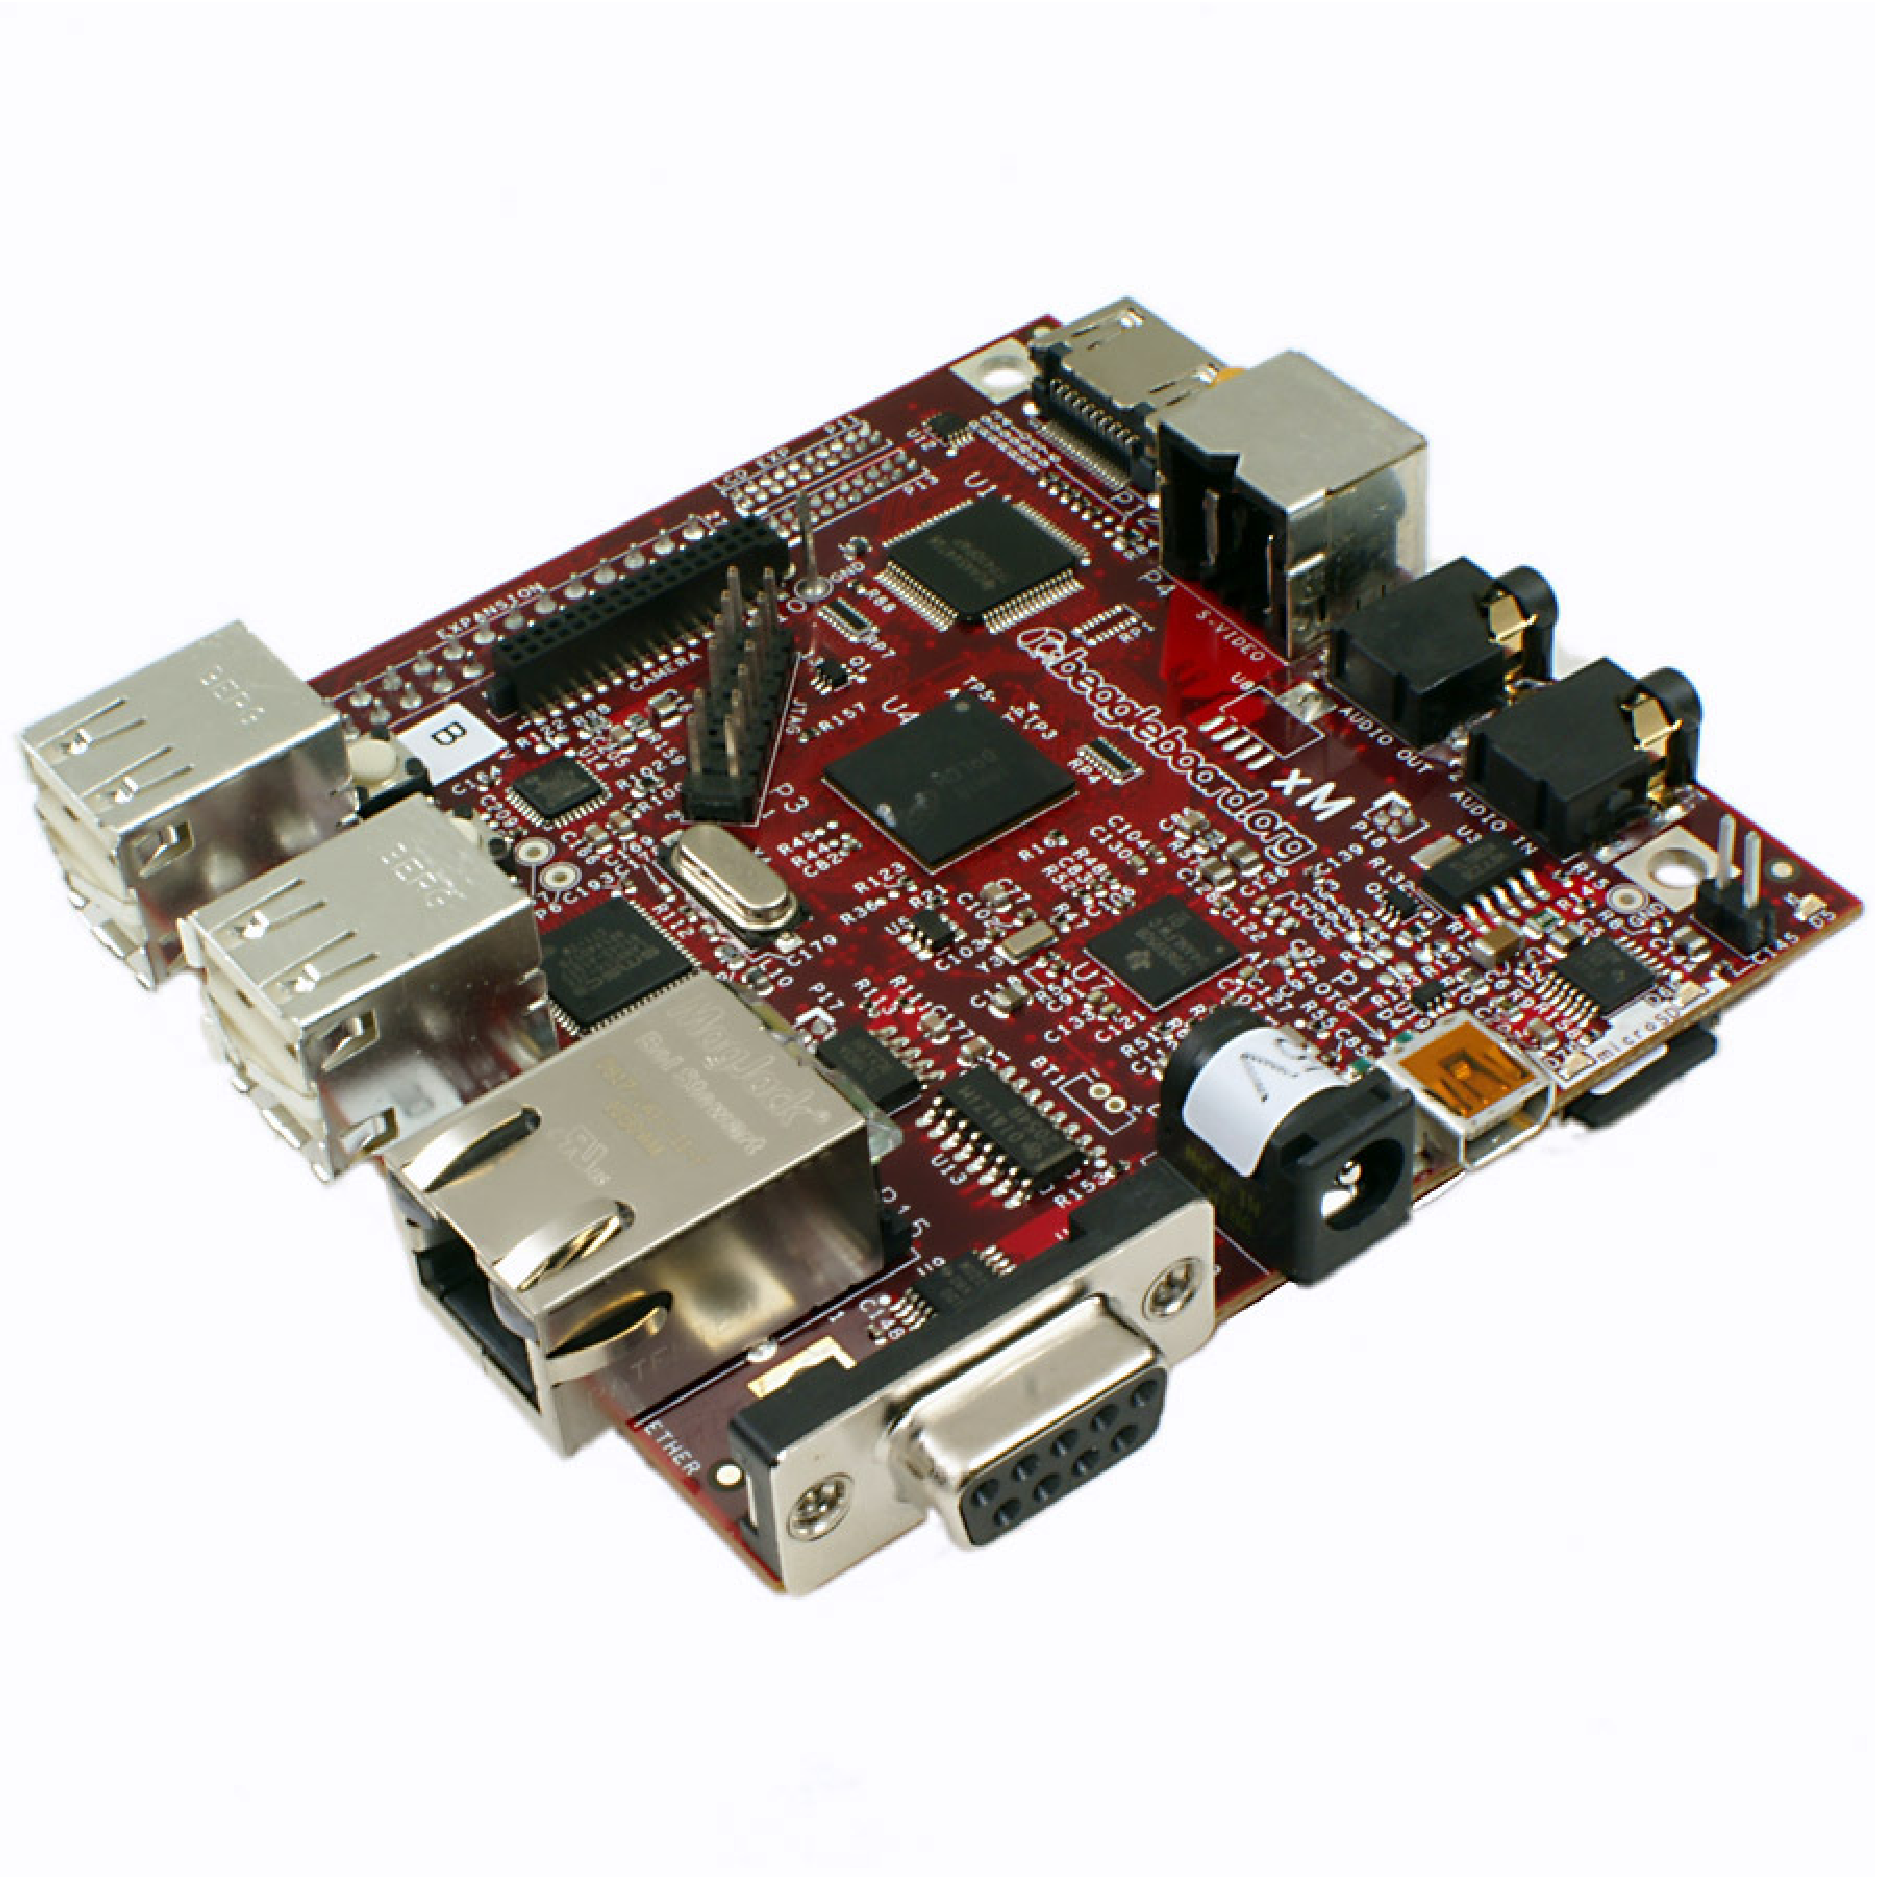
\includegraphics[width=0.35\textwidth]{./pics_eleccion_hardware/beagle.pdf}
\vspace{-30pt}
	\caption{Beagleboard}
	\label{fig:beagleboard}
\end{wrapfigure}


Adem\'as de la plataforma f\'isica, deben seleccionarse componentes electr\'onicos capaces de procesar la informaci\'on proveniente de los sensores, computar y ejecutar los algoritmos de control, y generar las se\~nales necesarias para transmitir las instrucciones a los motores.\\

La soluci\'on implementada se basa en la plataforma de desarrollo \emph{Beagleboard}. Esta plataforma posee un microprosesador TI ARM Cortex A8 de 1GHz y un DSP TMS320C64x+ de 800MHz. La memor\'ia RAM es de 512 Mb. No tiene memoria no vol\'atil, pero soporta tarjetas SD de hasta 4GB y es posible conectar memorias flash USB. Ver figura \ref{fig:beagleboard}.

\subsection*{Dimensiones y peso}

Cuanto menor sean las dimensiones y peso de la placa elegida, mayor carga \'util quedar\'a disponible. El peso total de la BeagleBoard con una bater\'ia, diseñada especialmente alimentarla es de aproximadamente 200 gramos, y sus dimensiones son de $10cm\times8.5cm\times5cm$. La autonom\'ia de dicha bater\'ia es de aproximadamente 2 horas.

\subsection*{Sistema Operativo, Puertos y I/O}

La BeagleBoard ofrece la posilibidad de cargar un kernel de \emph{Linux} desde una tarjeta SD. El sistema operativo permite:
\begin{itemize}
\item Comunicaci\'on a trav\'es de una interfaz ethernet.
\item Conexi\'on de cuatro dispositivos USB de manera simult\'anea.
\item Debugging a trav\'es de un puerto serie.
\item Uso de bibliotecas para visi\'on por computadora. 
\item Compatibilidad con m\'odulos de c\'amaras VGA.
\end{itemize}

Existen \textit{drivers} que permiten agregar una interfaz para WiFi conectando un m\'odulo USB (Belkin wireless G).

La BeagleBoard cuenta con un puerto de expansi\'on de 28 pines de proposito general. Los pines 23 y 24 de dicho puerto pueden ser configurados para exponer un puerto $I^2C$, fundamental para enviar comandos a los ESC. Los pines 23 y 24 corresponden a las lineas de datos y al reloj respectivamente. Por otra parte, los pines 8 y 6 pueden ser configurados para funcionar como pines de transmisi\'on y recepci\'on de un puerto serie, esto ser\'a fundamental para la comunicaci\'on con algunos de los sensores.

\section{Instrumentaci\'on}

Para poder controlar el sistema es importante poder conocer los valores que toman las variables de estado del mismo. Como se ver\'a en el cap\'itulo sobre el desarrollo del modelo f\'isico del cuadric\'optero, las variables que se deben conocer son:

\begin{itemize}
\item La orientaci\'on.
\item La posici\'on.
\item La velocidad.
\item La velocidad angular.
\end{itemize}

Por dicho motivo resulta imprescindible dotar al sistema de sensores capaces de medir dichas magnitudes, directa o indirectamente. Se compararon distintas alternativas comerciales, finalmente se opt\'o por un dispositivo que integra varios sensores y un GPS.
\subsection{IMU}

\subsubsection{Aceler\'ometro}
\label{acelerometro}

Un aceler\'ometro es un dispositivo capaz de medir su aceleraci\'on propia en el marco de referencia de un sistema en ca\'ida libre. Se encarga de procesar las medidas, y convertirlas a una se\~nal el\'ectrica (puede ser anal\'ogica o digital).\\
%TODO q onda con esto?
%Esto implica que el dispositivo no mide siempre su cambio de velocidad en el espacio. Por ejemplo, la medida de un aceler\'ometro en ca\'ida libre ser\'a cero a pesar de que su velocidad crezca, de la misma forma se puede observar que un aceler\'ometro en reposo respecto de la Tierra, no dar\'a una medida nula, sino que por el contrario medir\'a como aceleraci\'on \textit{g}.\\

Existen diversos tipos de aceler\'ometros. Se eligi\'o trabajar con un aceler\'ometro contenido en un circuito integrado, tecnolog\'ia MEMS. Los aceler\'ometros basados en esta tecnolog\'ias miden cambios internos de la transferencia de calor causada por la aceleraci\'on, ofreciendo ventajas significativas sobre el empleo de una estructura tradicional s\'olida de masas de prueba.\\

Se opt\'o por utilizar tecnolog\'ia MEMS fundamentalmente por tama\~no, peso y costo. Los mismos son m\'as peque\~nos, livianos y baratos que otras tecnolog\'ias.\\



El aceler\'ometro cumple dos roles fundamentales:
\begin{enumerate}
\item Bajo la hip\'otesis de que las aceleraciones a las cuales se ver\'a sometido el sistema \textbf{no} son comparables con $g$, sirve para determinar los \'angulos de Pitch y de Roll. En la figurea \ref{fig:acc_pitch} se ilustra la forma de lograr esto para el \'angulo de Pitch. Las ecuaciones utilizadas pueden encontrarse en \ref{chap:Software}.
\item Permite obtener una estimaci\'on de la velocidad, integrando su medida.  
\end{enumerate}

 \begin{figure}
	\centering
	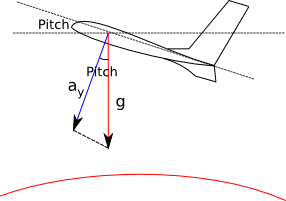
\includegraphics[width=0.5\textwidth]{./pics_eleccion_hardware/euler.png}
	\vspace{-10pt}
	\caption{Determinaci\'on del \'angulo de Pitch}
	\label{fig:acc_pitch}
\end{figure}
\subsubsection{Gir\'oscopo}
\label{giro}

Un gir\'oscopo es un instrumento capaz de medir la velocidad angular de un sistema solidario a si mismo respecto a un sistema inercial. Las mismas restricciones sobre tama\~no, peso y costo que se aplicaban para el aceler\'ometro se aplican aqu\'i. Se vuelve a optar por tecnolog\'ia MEMS.\\ 

Desde el punto de vista te\'orico, procesando la informaci\'on obtenida a partir del aceler\'ometro y del gir\'oscopo y partiendo de condiciones iniciales conocidas, se puede conocer, en todo momento, la posici\'on del sistema y su orientaci\'on. En la pr\'actica, sin embargo, esto no es as\'i, ya que todas las medidas tienen un cierto error. Para obtener la orientaci\'on y la posici\'on en cada instante se debe integrar y, por lo tanto, se integra tambi\'en el error cometido. Esto produce una acumulaci\'on de errores que afecta, de forma considerable, el resultado final luego de cierta cantidad de muestras. Este problema se puede resolver integrando un GPS. Este \'ultimo permitir\'ia, cada cierto intervalo de tiempo, contar con una medida absoluta para comparar contra los resultados obtenidos de la integral de las medidas del aceler\'ometro y del gir\'oscopo, permitiendo corregir errores debido a la deriva por integraci\'on del error.

\subsubsection{Sensor de presi\'on}

El GPS, mencionado en la secci\'on anterior, provee una estimaci\'on de la altura absoluta, pero es poco precisa. Depende fuertemente de la cantidad de sat\'elites disponibles y se ve fuertemente deteriorada por el efecto del rebote de las ondas en estructuras cercanas (en especial por los rebotes en el piso, que deterioran la precisi\'on en la medida de altura cuando se est\'a muy cerca del suelo). Por este motivo es necesario contar con otra fuente de informaci\'on. Se opt\'o por incorporar un bar\'ometro que, midiendo la presi\'on absoluta, permite determinar la altura del cuadric\'optero en forma independiente al resto de los sensores.

\subsubsection{Magnet\'ometro}

El \textit{drift} en la estimaci\'on del \'angulo de Yaw a partir de la integraci\'on de datos del gir\'oscopo y la falta de una referencia absoluta en dicha estimaci\'on, se resuelven agregando un magnet\'ometro. Permite ubicar el norte magn\'etico (medida absoluta), complementando la informaci\'on diferencial obtenida del gir\'oscopo.

\subsubsection{Sensor de temperatura}

El control del sistema no depende directamente de la temperatura, pero la instrumentaci\'on presenta una dependencia con (y por ende tendr\'a errores asociados a) la temperatura. El contar con un sensor de temperatura permitir\'a utilizar una calibraci\'on que tome en cuenta dicha dependencia.\\

La Mongoose 9DoF IMU (\ref{fig:mongoose}) posee todos los sensores que se han nombrado hasta aqu\'i, excepto el GPS. Las caracter\'isticas de dichos sensores se resumen en el anexo \ref{chap:anexo_mongoose}. Posee adem\'as un microprocesador sencillo de programar, lo que permite realizar un preprocesamiento de los datos antes de la estimaci\'on del estado. Las modificaciones realizadas al c\'odigo original se explican en el anexo \ref{chap:codigo}.

\begin{figure} 
  \vspace{-40pt}
  \centering
  \subfloat[Mongoose]{\label{fig:mongoose}
  \vspace{-40pt}
  		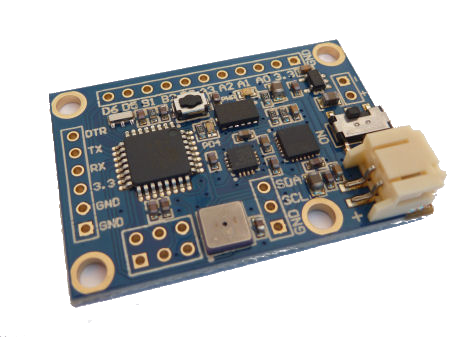
\includegraphics[width=0.3\textwidth]
  			{./pics_eleccion_hardware/Mongoose.png}}\hspace{2cm}
  \subfloat[Canmore GT-730F]{\label{fig:gps} 
  		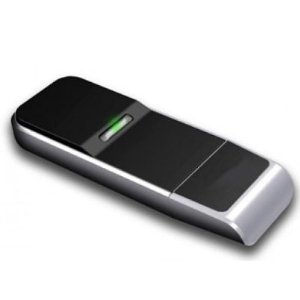
\includegraphics[width=0.3\textwidth]
  			{./pics_eleccion_hardware/gps.jpg}}
  
  \caption{Instrumentaci\'on}
  \label{fig:intrumentacion}
\end{figure}

\subsection{GPS}

La elecci\'on del GPS se bas\'o fundamentalmente en lograr la simplicidad del sistema. Exist\'ian muchas opciones, placas de diversos tama\~nos, con distintos tipos de antenas, pero todas con especificaciones similares.\\

Se opt\'o por utilizar un GPS \textit{Canmore GT-730F}, como el mostrado en la figura \ref{fig:gps}. Dentro de un margen de precios razonable las caracter\'isticas de los distintos GPS comerciales no difieren considerablemente en lo que refiere a tasa de muestreo, resoluci\'on y exactitud. La raz\'on fundamental para elegir dicho instrumento sobre otros fue la facilidad de conexi\'on ya que permite utilizar los puertos USB de la plataforma a cargo de la inteligencia y los drivers existentes para linux. \\ 

\subsection{Resumen de sensores}
\label{sec:hardware:resumen-de-sensores}

A continuaci\'on se presenta un resumen de las prestaciones de los sensores a utilizar, en la configuraci\'on en la que se utilizaron. Por m\'as detalles referirse a \ref{chap:anexo_mongoose}.

\begin{table}[H]
\begin{center}
\rowcolors{1}{gray!20}{}
\begin{tabular}{|p{3.5cm}|p{2.05cm}|p{2.05cm}|}
\hline
 & Dato nuevo & Resoluci\'on \\
\hline
Aceler\'ometro XY & 10ms (x2)& 4mg\\
\hline
Aceler\'ometro Z  & 10ms (x2)& 4mg\\
\hline
Gir\'oscopo XY  & 10ms (x2)& 0.07 $^\circ/s$\\
\hline
Gir\'oscopo Z  & 10ms (x2)& 0.07 $^\circ/s$\\
\hline
Bar\'ometro  & 10ms & 1Pa\\
\hline
Magnet\'ometro XY  & 10ms  (x2)& 5 mGa\\
\hline
Magnet\'ometro Z  & 10ms (x2)& 5 mGa\\
\hline
GPS  & 1s & - \\
\hline
\end{tabular}
\label{tab:hardware:resumen-sensores}
\end{center}
\end{table}


\end{document}

%Algunos layouts para poner im\'agnenes. Copien y peguen nom\'as. Hay figura com\'un, dos figuras en 1 onda fig 3a y 3b, wrapfigures y una matriz de figuras. Ta bueno, todas quedan lindas y andan bien.
%
%\begin{figure}[h!]
%	\centering
%	\includegraphics[width=0.75\textwidth]{./pics_eleccion_hardware/		.eps}
%	\caption{		}
%	\label{fig:		}
%\end{figure}
%
%\begin{figure} [h!]
%  \centering
%  \subfloat[caption 1]{\label{fig:		}
%  		\includegraphics[width=0.45\textwidth]
%  			{./pics_eleccion_hardware/		.eps}}
%  \subfloat[caption 2]{\label{fig:		} 
%  		\includegraphics[width=0.45\textwidth]
%  			{./pics_eleccion_hardware/ 		.eps}}
%  \caption{Caption general}
%  \label{fig:	label general	}
%\end{figure}
%
%\begin{wrapfigure}{l}{0.6\textwidth}
%  \vspace{-20pt}
%  \begin{center}
%    \includegraphics[width=0.45\textwidth]
%    	{./pics_eleccion_hardware/		.eps}
%  \end{center}
%  \vspace{-20pt}
%  \caption{		}
%  \label{ 		}
%  \vspace{-10pt}
%\end{wrapfigure}
%
%\begin{figure} [h!]
%  \begin{center}
%    \begin{tabular}{cc}
%      \resizebox{50mm}{!}
%      	{\includegraphics{./pics_eleccion_hardware/ 	.eps}} &
%      \resizebox{50mm}{!}
%      	{\includegraphics{./pics_eleccion_hardware/	.eps}} \\
%      \resizebox{50mm}{!}
%      	{\includegraphics{./pics_eleccion_hardware/	.eps}} &
%      \resizebox{50mm}{!}
%      	{\includegraphics{./pics_eleccion_hardware/	.eps}} \\
%    \end{tabular}
%    \caption{ 		}
%    \label{ 		}
%  \end{center}
%\end{figure}